\documentclass{article}
\usepackage[margin=0.5in]{geometry}
\usepackage{pgfplots}
\usepackage{tabto}
\pgfplotsset{width=10cm,compat=1.3}

\begin{document}
	CSci242 Assignment III: Graph\newline
	\tab \tab Author: Grant Haataja\newline
	\tab \tab Spring 2019: 04/08/2019\newline

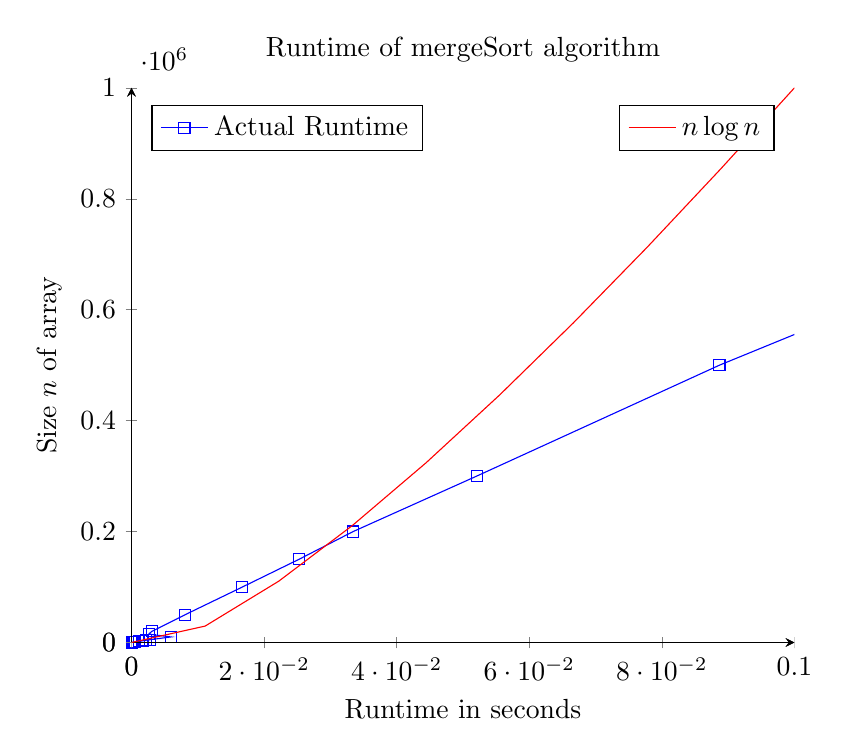
\begin{tikzpicture}% coordinates
\begin{axis}[
	title={Runtime of mergeSort algorithm},
	axis lines = left,
	xlabel = Runtime in seconds,
	ylabel = {Size $n$ of array},
	xmin=0, xmax=.1,
	ymin=0, ymax=1000000,
	legend pos=north west,
]

\addplot[
	domain=0:0.5,
	color=blue,
	mark=square,
]
coordinates {
(0.000009,10)(0.000010,20)(0.000015,30)(0.000019,40)(0.000023,50)(0.000038,100)(0.000061,150)(0.000079,200)(0.000109,250)(0.000216,500)(0.000345,750)(0.000468,1000)(0.001111,2000)(0.001648,3000)(0.002163,4000)(0.002783,5000)(0.005951,10000)(0.002595,15000)(0.003047,20000)(0.008066,50000)(0.016718,100000)(0.025265,150000)(0.033428,200000)(0.052069,300000)(0.088692,500000)(0.109136,600000)(0.161426,900000)(0.181441,1000000)(0.277971,1500000)(0.374413,2000000)
};
\addlegendentry{Actual Runtime}

\end{axis}

\begin{axis}[
axis lines = left,
	xtick={0},
	ytick={0},
legend pos=north east,
]
\addplot [
domain=0:20,
samples=10,
color=red,
]
{x * log10(x)};
\addlegendentry{$n\log n$}

\end{axis}
\end{tikzpicture}

\vspace{.2in}
We can see that there is a significant difference between the theoretical graph of the algorithm (red) and the actual plotted data points (blue). This is likely due to the fact that the computer the program was run on is a few years old and the processing speed decreases relative to the theoretical speed as the size of the problem increases. 
\end{document}